\section{Resultados}
\label{chap:resultados}

Esta seção apresenta os principais achados obtidos a partir dos experimentos conduzidos. Inicialmente, descrevemos uma análise exploratória detalhada do conjunto de dados, seguida pelo diagnóstico estatístico das variáveis. Em seguida, relatamos o desempenho dos diferentes modelos ajustados, comparando-os de forma sistemática segundo os critérios estabelecidos na metodologia.

\subsection{Análise Exploratória e Diagnóstico dos Dados}


O conjunto \textit{Real Estate Valuation} apresenta preditores em escalas muito distintas, o que justifica a avaliação sistemática de diferentes esquemas de normalização. A estatística descritiva (Tabela~\ref{tab:eda_describe}) evidencia contrastes relevantes, uma vez que a distância à estação de metrô (MRT) apresenta forte assimetria à direita, com média de $1084$ e desvio padrão de $1262$, ao passo que o número de lojas de conveniência constitui uma variável discreta de baixa cardinalidade.


\begin{table}[h!]

    \centering

    \caption{Sumário descritivo das variáveis preditoras.}

    \label{tab:eda_describe}

    \resizebox{\textwidth}{!}{%

    \begin{tabular}{lcccccc}

        \toprule

        & \textbf{X1 transaction date} & \textbf{X2 house age} & \textbf{X3 distance to MRT} & \textbf{X4 \# convenience stores}& \textbf{X5 latitude} & \textbf{X6 longitude} \\

        \midrule

        count & 414 & 414 & 414 & 414 & 414 & 414 \\

        mean  & 2013.15 & 17.71 & 1083.89 & 4.09 & 24.97 & 121.53 \\

        std   & 0.28 & 11.39 & 1262.11 & 2.95 & 0.01 & 0.02 \\

        min   & 2012.67 & 0 & 23.38 & 0 & 24.93 & 121.47 \\

        25\%  & 2012.92 & 9.03 & 289.32 & 1 & 24.96 & 121.53 \\

        50\%  & 2013.17 & 16.10 & 492.23 & 4 & 24.97 & 121.54 \\

        75\%  & 2013.42 & 28.15 & 1454.28 & 6 & 24.98 & 121.54 \\

        max   & 2013.58 & 43.80 & 6488.02 & 10 & 25.01 & 121.57 \\

        \bottomrule

    \end{tabular}
    }

\end{table}



A matriz de correlação (Figura~\ref{fig:eda_corr}) confirma associações lineares consistentes com a literatura. Observa-se uma correlação negativa elevada entre o preço e a distância ao MRT, com $r \approx -0.67$, além de correlações positivas moderadas com o número de lojas ($r \approx 0.57$) e com as coordenadas geográficas (latitude, $r \approx 0.55$; longitude, $r \approx 0.52$). Também se destaca a alta correlação entre os próprios preditores espaciais, como distância ao MRT e longitude ($r \approx -0.81$), o que sugere a presença de colinearidade, aspecto relevante para a estabilidade de modelos lineares.



\begin{figure}[h!]

    \centering

    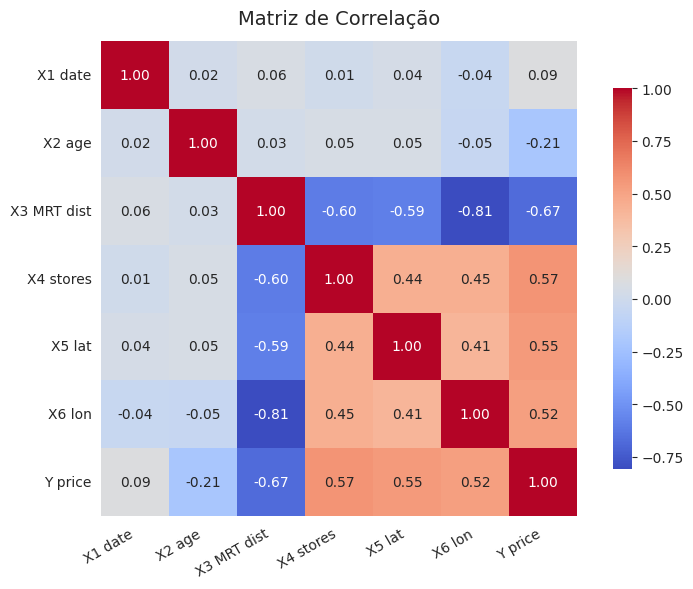
\includegraphics[width=0.8\textwidth]{figuras/eda_corr_heatmap.png} % Substitua pelo caminho da sua figura

    \caption{Matriz de correlação entre as variáveis preditoras e a variável alvo (preço).}

    \label{fig:eda_corr}

\end{figure}



%--------------------------------------------------------------------

% Análise por Modelo (Estrutura Padronizada)

%--------------------------------------------------------------------

\subsection{Análise de Desempenho dos Modelos Implementados}


A seguir, detalha-se o desempenho dos melhores modelos de cada classe, selecionados conforme o critério lexicográfico (\emph{Hit@10} $\rightarrow$ \emph{Hit@20} $\rightarrow$ $R^2$ $\rightarrow$ RMSE) aplicado sobre os resultados da validação cruzada.

\subsubsection{Modelo de Mínimos Quadrados (MQ)}

O melhor modelo linear foi obtido com normalização robusta, baseada no intervalo interquartil, e regularização \textit{Ridge} ($\lambda=0.5$). No conjunto de teste, o modelo apresentou desempenho satisfatório, com $\mathrm{RMSE}=7.06$ e $R^2=0.689$.

A Figura~\ref{fig:mqo_disp_hist} evidencia um bom alinhamento entre os valores preditos e observados, ainda que se note uma tendência à subestimação em imóveis de maior valor. Esse comportamento, frequentemente encontrado em dados imobiliários, sugere a presença de heterocedasticidade, já que a variância do erro tende a crescer com o preço do imóvel. O histograma dos resíduos de treino reforça essa interpretação, exibindo uma cauda longa à direita, associada principalmente a \textit{outliers} de alto valor. A análise formal por meio do teste de Shapiro–Wilk confirmou a ausência de normalidade nos resíduos ($W=0.819$, $p<10^{-4}$), em consonância com a assimetria previamente observada.

Apesar dessas limitações, a correlação entre valores observados e preditos (Tabela~\ref{tab:mqo_corr}) mostrou-se elevada e consistente tanto no treino quanto no teste, indicando boa generalização. Esse resultado reforça que a combinação de normalização robusta (IQR) e regularização L2 estabilizou a estimação frente à colinearidade e aos \textit{outliers}, mantendo coeficientes interpretáveis e coerentes com o domínio (Tabela~\ref{tab:mqo_coef}). Os coeficientes referem-se às variáveis preditoras na escala normalizada por IQR.



\begin{figure}[h!]

    \centering

    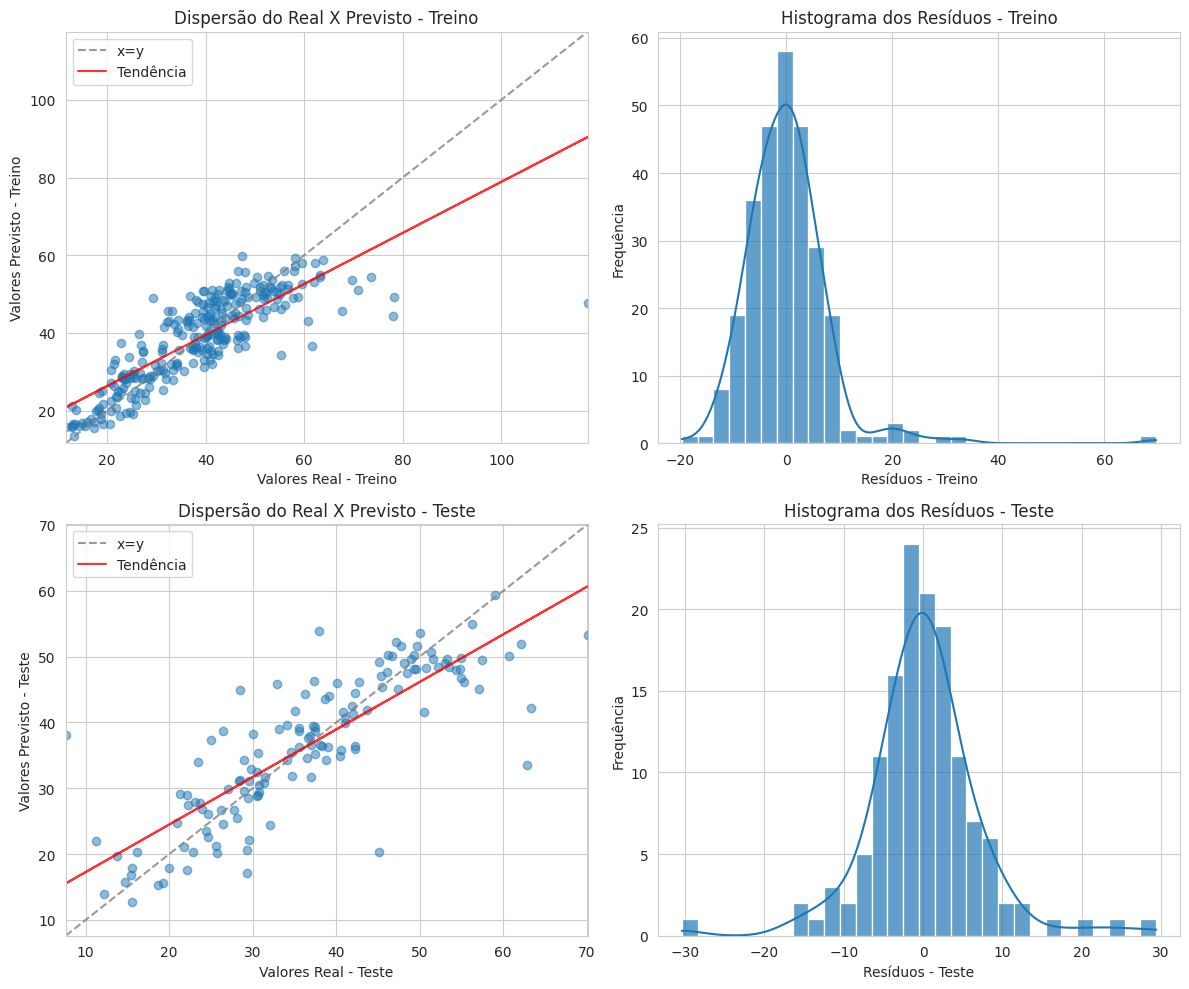
\includegraphics[width=0.75\textwidth]{figuras/mqo_dispersao_hist.png} % Substitua pelo caminho da sua figura

    \caption{MQ: Dispersão observado vs. predito e histograma dos resíduos (treino/teste).}

    \label{fig:mqo_disp_hist}

\end{figure}


\begin{table}[h!]

    \centering

    \caption{MQ: Correlação ($r$) entre valores observados e preditos.}

    \label{tab:mqo_corr}

    \begin{tabular}{lc}

        \toprule

        Conjunto & Correlação $r$ \\

        \midrule

        Treino & 0.816 \\

        Teste  & 0.831 \\

        \bottomrule

    \end{tabular}

\end{table}



\begin{table}[h!]

    \centering

    \caption{MQ: Coeficientes estimados do modelo Ridge ($\lambda=0.5$) com normalização robusta.}

    \label{tab:mqo_coef}

    \begin{tabular}{lc}

        \toprule

        \textbf{Variável} & \textbf{Coeficiente ($b_i$)} \\

        \midrule

        Intercepto ($b_0$) & 40.42 \\

        X1: Data da transação & 6.01 \\

        X2: Idade do imóvel & -8.57 \\

        X3: Distância até estação de MRT & -23.18 \\

        X4: Número de lojas de conveniência & 4.82 \\

        X5: Latitude & 14.67 \\

        X6: Longitude & 2.61 \\

        \bottomrule

    \end{tabular}

\end{table}

% ... (As tabelas de coeficientes e outras podem ser mantidas aqui se desejado)


\subsubsection{Perceptron Logístico (PS)}

O melhor modelo de Perceptron, configurado a função de ativação logística, foi treinado a partir de dados padronizados por z-score, empregando taxa de aprendizado de $0.005$ e $300$ épocas de treinamento. No conjunto de teste, o desempenho obtido correspondeu a $\mathrm{RMSE}=7.79$ e $R^2=0.622$.

A análise das dispersões apresentadas na Figura~\ref{fig:pl_disp_hist} evidencia uma compressão na faixa de predições, fenômeno característico de funções de ativação sigmoides, que tende a provocar subestimação dos valores mais extremos. O padrão dos resíduos mostrou-se semelhante ao verificado no modelo MQ, destacando-se a presença de caudas pesadas e assimetria à direita no conjunto de treinamento. A avaliação estatística por meio do teste de Shapiro--Wilk rejeitou a hipótese de normalidade ($W=0.822$, $p<10^{-4}$), resultado coerente com a assimetria observada. 

As correlações reportadas na Tabela~\ref{tab:pl_corr} revelam associações moderadamente altas entre valores observados e preditos, ainda que inferiores às verificadas no modelo MQ. A proximidade dos resultados entre os conjuntos de treino e teste sugere ausência de sobreajuste relevante, reforçando a estabilidade do modelo. 

Em síntese, a padronização dos dados mostrou-se determinante para assegurar a convergência do algoritmo. Apesar de capturar adequadamente a tendência geral do fenômeno, as limitações inerentes à função de ativação logística comprometeram a capacidade de previsão em faixas de preços mais elevados, o que resultou em desempenho inferior ao do modelo linear regularizado.

\begin{figure}[h!]

    \centering

    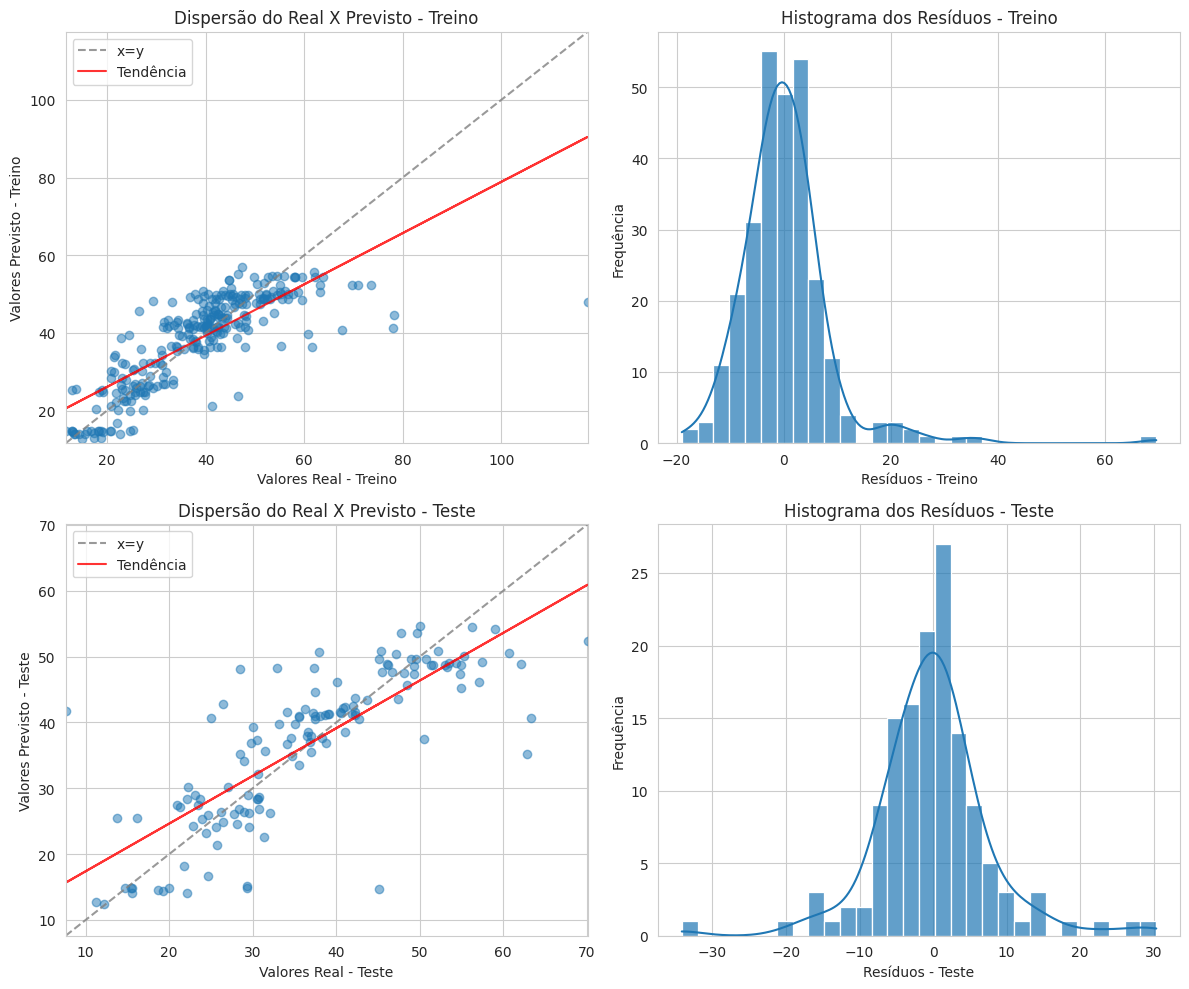
\includegraphics[width=0.75\textwidth]{figuras/pl_dispersao_hist.png} % Substitua pelo caminho da sua figura

    \caption{PS: Dispersão observado vs. predito e histograma dos resíduos (treino/teste).}

    \label{fig:pl_disp_hist}

\end{figure}


\begin{table}[h!]

    \centering

    \caption{PS: Correlação ($r$) entre valores observados e preditos.}

    \label{tab:pl_corr}

    \begin{tabular}{lc}

        \toprule

        Conjunto & Correlação $r$ \\

        \midrule

        Treino & 0.793 \\

        Teste  & 0.797 \\

        \bottomrule

    \end{tabular}

\end{table}



\subsubsection{MLP com Uma Camada Oculta (MLP-1C)}

A melhor MLP com uma camada oculta empregou padronização pelo z-score, função de ativação \texttt{leaky\_relu}, 256 neurônios, e foi treinada por 200 épocas com taxa de aprendizado $lr=0.005$. No conjunto de teste, o modelo alcançou $\mathrm{RMSE}=7.65$ e $R^2=0.635$, resultados que, embora satisfatórios, já antecipam limitações quando comparados ao \textit{baseline} linear.

A análise gráfica (Figura~\ref{fig:mlp1_disp_hist}) confirma um alinhamento geral adequado, mas evidencia tendência de subestimação nos valores extremos. Esse comportamento decorre da maior capacidade representacional do modelo, possibilitada pelos 256 neurônios na camada oculta, que lhe permitiu ajustar-se aos dados de treinamento.

\begin{figure}[h!]

    \centering

    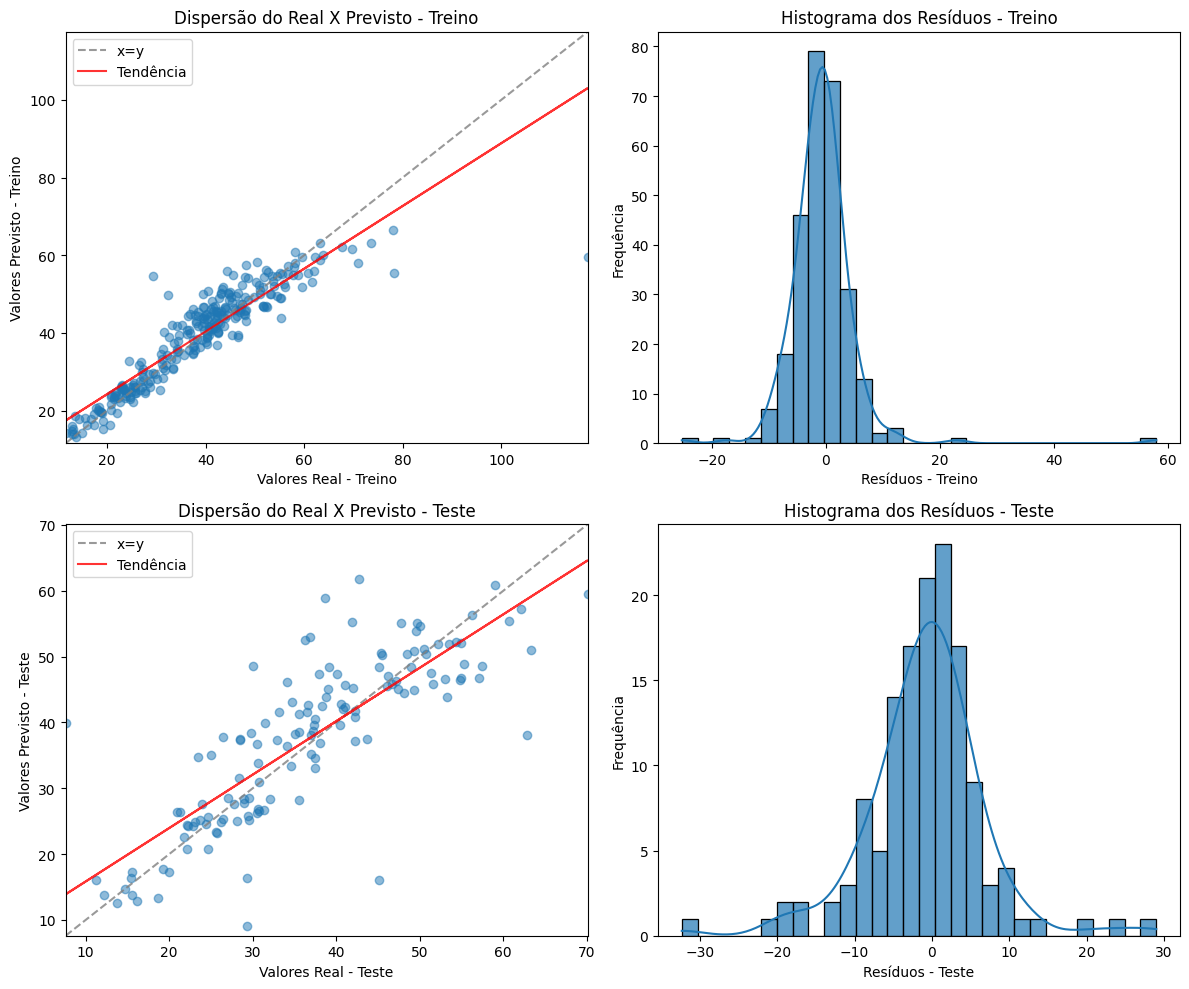
\includegraphics[width=0.75\textwidth]{figuras/mlp1_dispersao_hist.png} % Substitua pelo caminho da sua figura

    \caption{MLP-1C: Dispersão observado vs. predito e histograma dos resíduos (treino/teste).}

    \label{fig:mlp1_disp_hist}

\end{figure}


Essa hipótese é corroborada pela análise dos resíduos. O teste de Shapiro--Wilk rejeitou a normalidade ($W=0.745$, $p<10^{-4}$), indicando caudas mais pesadas do que as observadas nos demais modelos. De forma consistente, as correlações apresentadas na Tabela~\ref{tab:mlp1_corr} revelam diferença substancial entre treino ($r=0.911$) e teste ($r=0.818$), caracterizando a ocorrência de sobreajuste.

A combinação da função \texttt{leaky\_relu} com a elevada capacidade da camada oculta favoreceu a memorização de parte dos dados de treinamento. Embora tenha capturado a tendência geral do fenômeno, o modelo não superou o \textit{baseline} linear, o que indica que sua complexidade mostrou-se excessiva para o tamanho do conjunto de dados disponível.

\begin{table}[h!]

    \centering

    \caption{MLP-1C: Correlação ($r$) entre valores observados e preditos.}

    \label{tab:mlp1_corr}

    \begin{tabular}{lc}

        \toprule

        Conjunto & Correlação $r$ \\

        \midrule

        Treino & 0.911 \\

        Teste  & 0.818 \\

        \bottomrule

    \end{tabular}

\end{table}


\subsubsection{MLP com Duas Camadas Ocultas (MLP-2C)}

A melhor arquitetura com duas camadas ocultas, configurada com $[64, 32]$ neurônios, empregou normalização \textit{min--max}, função de ativação \texttt{tanh} e taxa de aprendizado $lr=0.01$. No conjunto de teste, o modelo apresentou $\mathrm{RMSE}=7.18$ e $R^2=0.679$, valores competitivos em relação ao baseline linear.

A análise gráfica (Figura~\ref{fig:mlp2_disp_hist}) revela um desempenho visualmente próximo ao obtido pelo modelo MQ, caracterizado por ajuste robusto, ainda que sujeito à heterocedasticidade presente nos dados. A inspeção dos resíduos confirmou essa limitação, uma vez que o teste de Shapiro--Wilk rejeitou a hipótese de normalidade ($W=0.804$, $p<10^{-4}$). As correlações reportadas na Tabela~\ref{tab:mlp2_corr} mostraram-se elevadas e bastante próximas entre treino ($r=0.841$) e teste ($r=0.828$), sugerindo que esta arquitetura, embora mais profunda, foi menos suscetível ao sobreajuste do que a MLP-1C, possivelmente em razão do menor número total de parâmetros.


\begin{figure}[h!]

    \centering

    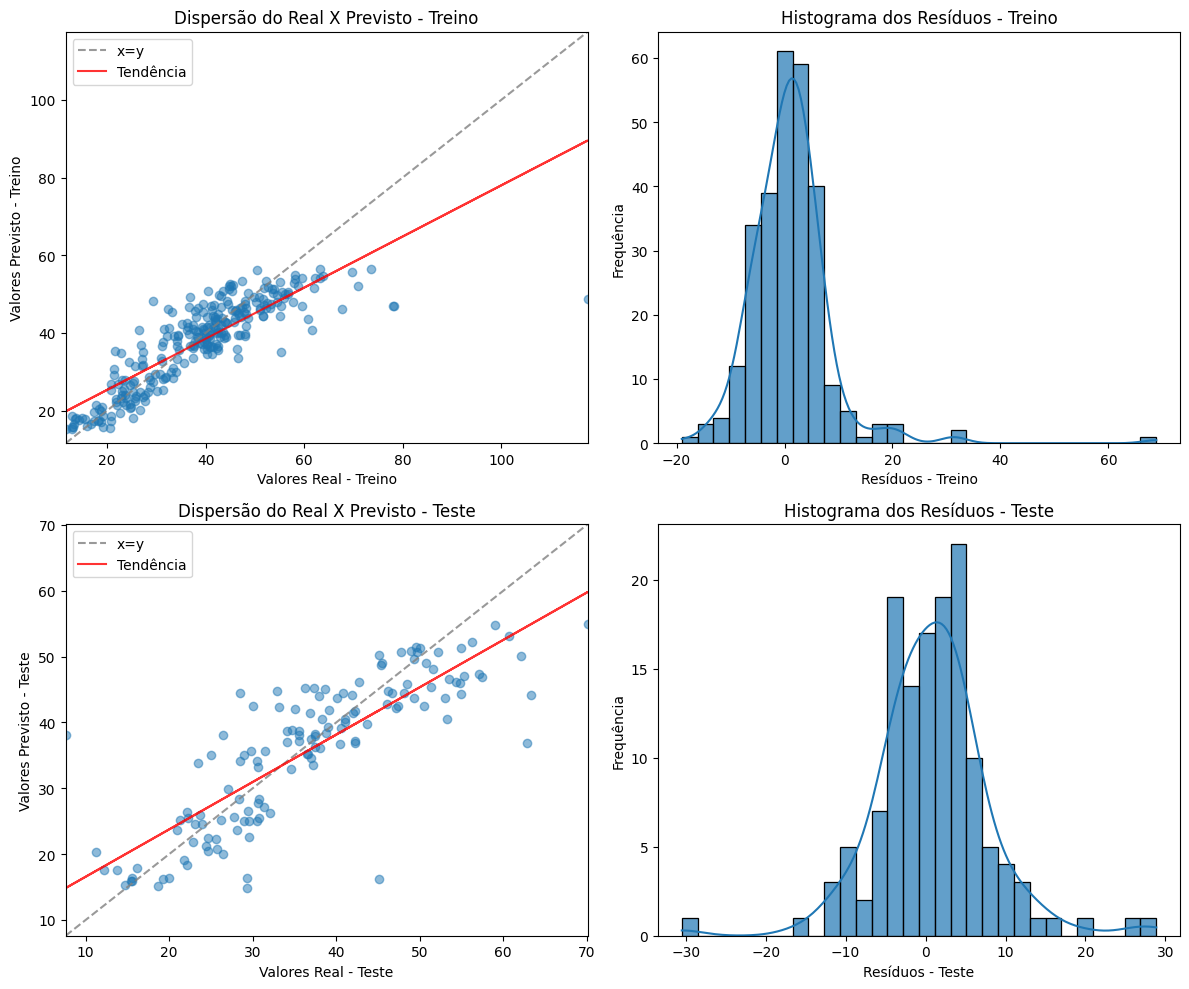
\includegraphics[width=0.75\textwidth]{figuras/mlp2_dispersao_hist.png} % Substitua pelo caminho da sua figura

    \caption{MLP-2C: Dispersão observado vs. predito e histograma dos resíduos (treino/teste).}

    \label{fig:mlp2_disp_hist}

\end{figure}

\begin{table}[h!]

    \centering

    \caption{MLP-2C: Correlação ($r$) entre valores observados e preditos.}

    \label{tab:mlp2_corr}

    \begin{tabular}{lc}

        \toprule

        Conjunto & Correlação $r$ \\

        \midrule

        Treino & 0.841 \\

        Teste  & 0.828 \\

        \bottomrule

    \end{tabular}

\end{table}


A combinação da normalização \textit{min--max} com a função de ativação \texttt{tanh} mostrou-se adequada para esta configuração, permitindo que o modelo atingisse desempenho competitivo e comparável ao do MQ. Esses resultados indicam que, neste problema, arquiteturas não lineares mais profundas podem reproduzir a eficácia de um modelo linear bem regularizado, sem necessariamente superá-lo.





\subsubsection{Random Forest (RF)}

O modelo de Random Forest, treinado a partir de dados padronizados, apresentou o melhor desempenho geral entre os algoritmos avaliados. No conjunto de teste, alcançou o menor erro ($\mathrm{RMSE}=6.69$) e o maior coeficiente de determinação ($R^2=0.721$), superando tanto os modelos lineares quanto as redes neurais analisadas.

A inspeção dos gráficos de dispersão (Figura~\ref{fig:rf_disp_hist}) evidencia o alinhamento mais consistente entre valores observados e preditos, com menor viés sistemático nos imóveis de maior valor. Esse comportamento reflete a capacidade intrínseca de modelos baseados em árvores de capturar interações não lineares e efeitos de ordem superior, aspecto que mostrou-se particularmente relevante neste problema.

\begin{figure}[h!]

    \centering

    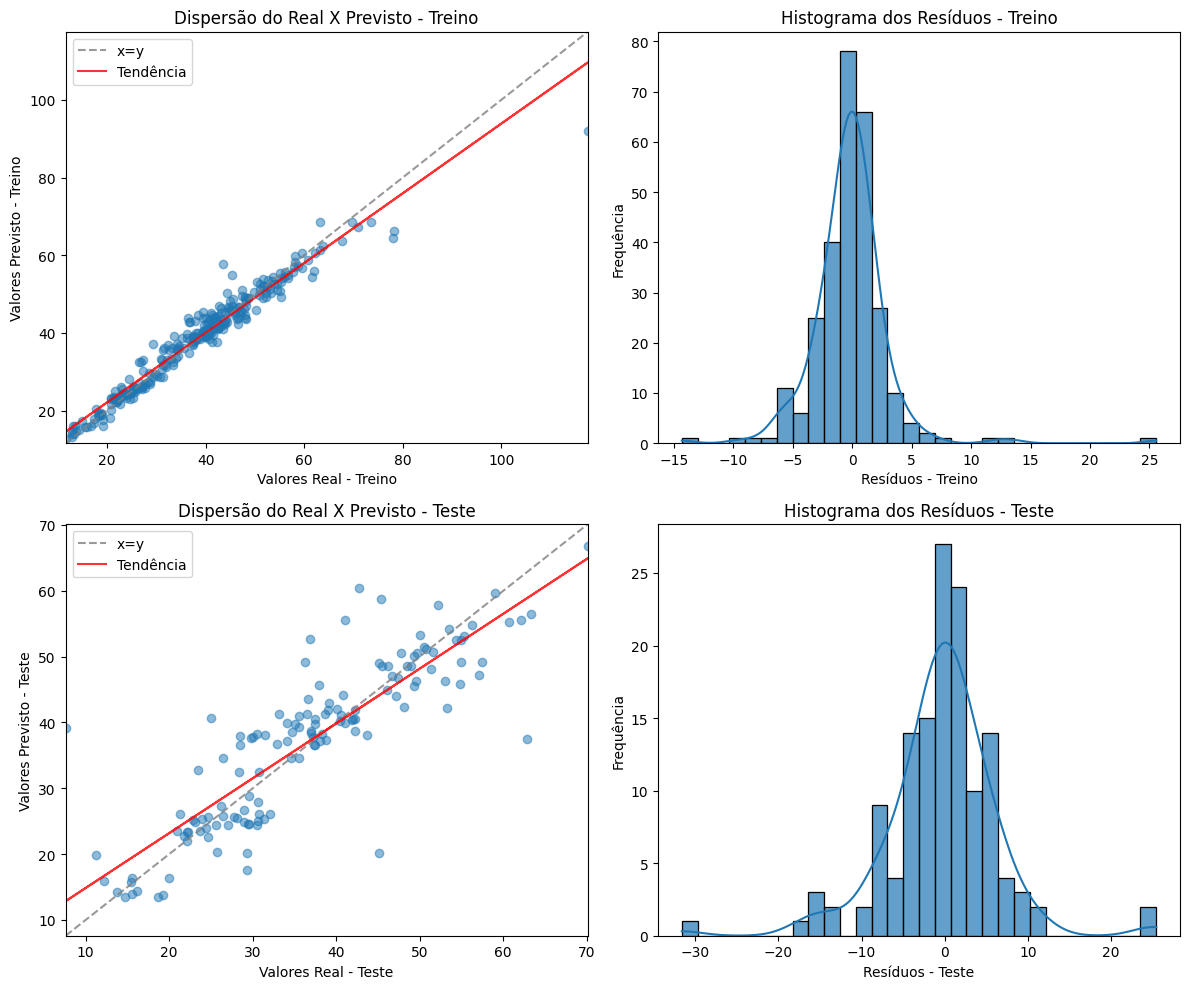
\includegraphics[width=0.75\textwidth]{figuras/rf_dispersao_hist.png} % Substitua pelo caminho da sua figura

    \caption{RF: Dispersão observado vs. predito e histograma dos resíduos (treino/teste).}

    \label{fig:rf_disp_hist}

\end{figure}

Embora a hipótese de normalidade dos resíduos tenha sido rejeitada pelo teste de Shapiro--Wilk ($W=0.828$, $p<10^{-4}$), tal pressuposto não constitui requisito para o funcionamento de algoritmos de árvores. As correlações confirmam o bom ajuste: no conjunto de teste, obteve-se $r=0.857$, o valor mais elevado entre todos os modelos, enquanto a correlação em treino ($r=0.976$) revela certo grau de sobreajuste. Esse comportamento, no entanto, é esperado no Random Forest e tende a ser atenuado pela agregação via \textit{bagging}, que contribui para a estabilidade do modelo.



\begin{table}[h!]

    \centering

    \caption{RF: Correlação ($r$) entre valores observados e preditos.}

    \label{tab:rf_corr}

    \begin{tabular}{lc}

        \toprule

        Conjunto & Correlação $r$ \\

        \midrule

        Treino & 0.976 \\

        Teste  & 0.857 \\

        \bottomrule

    \end{tabular}

\end{table}


Outro aspecto distintivo do Random Forest é a possibilidade de estimar a importância relativa das variáveis. A análise baseada em permutação indicou que a \textbf{distância ao MRT} constitui o preditor mais relevante, seguida pelo \textbf{número de lojas de conveniência} e pela \textbf{latitude}. Em contraste, a data da transação mostrou-se a variável menos informativa, o que está em consonância com os achados da análise exploratória. Esses resultados reforçam a evidência de que a localização é o fator predominante na determinação do preço dos imóveis neste conjunto de dados.



%--------------------------------------------------------------------

% Análise Comparativa e Discussão Final

%--------------------------------------------------------------------

\subsection{Análise Comparativa e Discussão com a Referência}

A Tabela~\ref{tab:shapiro_summary} sumariza os resultados do teste de Shapiro-Wilk para os resíduos de treino de todos os modelos. A rejeição por todos os modelos da hipótese de normalidade ($p<0.001$) é uma evidência de que os erros neste problema não seguem uma distribuição gaussiana, principalmente devido à presença de \textit{outliers}.


\begin{table}[h!]

\centering

\caption{Teste de Shapiro-Wilk para os resíduos de treino por modelo.}

\label{tab:shapiro_summary}

\begin{tabular}{@{}lcc@{}}

\toprule

\textbf{Modelo} & \textbf{Estatística $W$} & \textbf{$p$-valor} \\

\midrule

Mínimos Quadrados (MQ) & 0.819 & $< 10^{-4}$ \\

Perceptron Logístico (PS) & 0.822 & $< 10^{-4}$ \\

MLP-1C & 0.745 & $< 10^{-4}$ \\

MLP-2C & 0.804 & $< 10^{-4}$ \\

Random Forest (RF) & 0.828 & $< 10^{-4}$ \\

\bottomrule

\end{tabular}

\end{table}


Já a Tabela~\ref{tab:final_comparison} compara o desempenho dos modelos desenvolvidos neste trabalho com os resultados reportados por Yeh \& Hsu (2018). Os modelos de referência são MVR (\textit{Multiple Regression Valuation}), MLP e QCA (\textit{Qualitative Comparative Analysis with Case-Based Reasoning}).


\begin{table}[h!]
\centering
\caption{Comparativo de desempenho no conjunto de teste.}
\label{tab:final_comparison}
\resizebox{\textwidth}{!}{%
\begin{tabular}{lcccccc@{}}
\toprule
 \textbf{Modelo} & \textbf{RMSE} & \textbf{$R^2$} & \textbf{Hit@10\%} & \textbf{Hit@20\%} & \textbf{Preço Médio} & \textbf{RMSE/Preço Médio} \\
\midrule
 Random Forest (RF) & 6.69 & 0.721 & 56.9 & 78.80 & 50.30 & 0.133 \\
 GradBoost & 6.70 & 0.719 & 54.7 & 77.37 & 48.91 & 0.137 \\
 Mínimos Quadrados (MQ) & 7.06 & 0.689 & 52.6 & 79.60 & 49.37 & 0.143 \\
 MLP-2C (64, 32) & 7.18 & 0.679 & 46.7 & 83.20 & 45.16 & 0.159 \\
 SVR (RBF) & 8.05 & 0.595 & 48.9 & 70.0 & 50.41 & 0.159 \\
 MLP-1C (256) & 7.65 & 0.635 & 46.7 & 78.10 & 47.52 & 0.161 \\
 Perceptron Logístico (PS) & 7.79 & 0.622 & 54.0 & 75.20 & 47.21 & 0.165 \\
\midrule
 QCA (Referência) & 6.85 & 0.582 & 48.1 & 78.0 & 36.05 & 0.190 \\
 MLP (Referência) & 7.12 & 0.541 & 45.9 & 76.10 & 35.60 & 0.200 \\
 MVR (Referência) & 8.04 & 0.392 & 39.1 & 68.70 & 35.89 & 0.224 \\
\bottomrule
\end{tabular}}
\end{table}

É notável que múltiplos modelos desenvolvidos neste estudo superaram os benchmarks do artigo de referência em métricas como $R^2$ e \emph{Hit@k}. O modelo Random Forest demonstrou um desempenho superior ao melhor modelo de referência. Até mesmo nosso modelo linear (MQ), superou significativamente a MLP da referência.

Essas diferenças podem ser atribuídas ao nosso protocolo mais extensivo de busca de hiperparâmetros e à avaliação sistemática de diferentes esquemas de pré-processamento, que se mostraram cruciais para extrair o máximo de desempenho de cada classe de modelo. A principal conclusão é que, com um tratamento de dados e um ajuste de modelo cuidadosos, é possível obter resultados de ponta, com o modelo Random Forest se destacando como a abordagem mais precisa para este problema.

